\documentclass{article}
\usepackage{graphicx}
\usepackage[margin=1.5cm]{geometry}
\usepackage{amsmath}

\begin{document}
\twocolumn

\title{Wednesday Warm Up: Unit 4, Circular Motion}
\author{Prof. Jordan C. Hanson}

\maketitle

\section{Memory Bank}

\begin{itemize}
\item $\Delta s = r \Delta \theta$
\item $\omega = \frac{\Delta \theta}{\Delta t}$ ... Definition of angular velocity
\item $v = r\omega $ ... Relationship between tangential velocity and angular velocity a distance $r$ from the center
\item $a_C = v^2/r = r \omega^2$ ... Centripetal acceleration\
\item $\omega = (2\pi)/T$ ... The orbital period, $T$, if $\omega$ is constant.
\item \textbf{Force of Gravity:} The force of gravity between two objects of masses $m_1$ and $m_2$ separated by a distance $r$ is
\begin{equation}
F_G = G \frac{m_1 m_2}{r^2} \label{eq:1}
\end{equation}
In Eq. \ref{eq:1}, $G = 6.67 \times 10^{-11}$ N m$^{2}$ kg$^{-2}$.
\end{itemize}

\section{Newton's Law of Gravity}

\begin{enumerate}
\item The mass of the Moon is estimated to be $7.35 \times 10^{22}$ kg, and orbits the Earth at a distance of 384,000 km.  Assuming that the centripetal force is provided by Eq. \ref{eq:1}, solve for the orbital period of the moon. \\ \vspace{3.5cm}
\item Suppose astronauts measured $g=1.625$ m s$^{-2}$ near the surface of the Moon.  We know the mass of the Earth is $5.97 \times 10^{24}$ kg, and that the radius of the Earth is 6371 km.  We also know that the radius of the Moon is 1737 km.  What is the mass of the Moon? \\ \vspace{3.5cm}
\item
Explain in your own words why the high tides of the Earth's oceans orient themselves as in Fig. \ref{fig:tide1}.  Recall that Newton's Law of Gravity depends on $1/r^2$.  \\ \vspace{2cm}
\item The spring tides are the highest high tides, and the neap tides are the lowest high tides.  Explain why this is the case using Fig. \ref{fig:tide2} and Newton's Law of Gravity.
\end{enumerate}

\begin{figure}
\centering
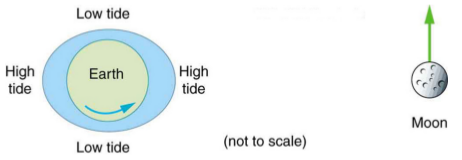
\includegraphics[width=0.45\textwidth]{tide1.png}
\caption{\label{fig:tide1} The tides of the Earth as they relate to the position of the Moon.}
\end{figure}

\begin{figure}
\centering
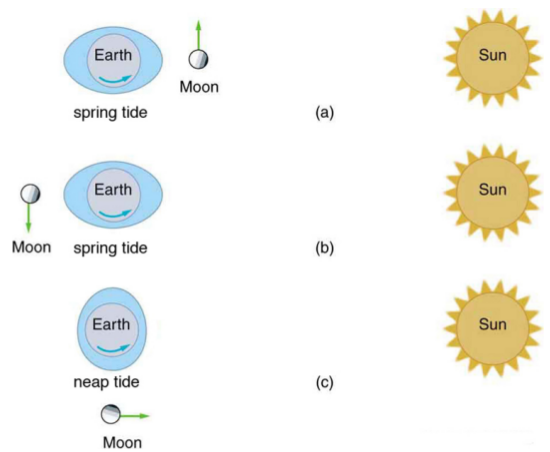
\includegraphics[width=0.4\textwidth]{tide2.png}
\caption{\label{fig:tide2} The spring and neap tides as they relate to the orientation of the Earth, Moon, and Sun.}
\end{figure}

\end{document}
